\documentclass[portrait,final]{baposter}
%\documentclass[a4shrink,portrait,final]{baposter}
% Usa a4shrink for an a4 sized paper.

\tracingstats=2

\usepackage{times}
\usepackage{calc}
\usepackage{graphicx}
\usepackage{amsmath}
\usepackage{amssymb}
\usepackage{relsize}
\usepackage{multirow}
\usepackage{bm}

\usepackage{graphicx}
\usepackage{wrapfig}
\usepackage{multicol}

\usepackage{pgfbaselayers}
\pgfdeclarelayer{background}
\pgfdeclarelayer{foreground}
\pgfsetlayers{background,main,foreground}

\usepackage{helvet}
%\usepackage{bookman}
\usepackage{palatino}

\usepackage{url}
\usepackage{fancyvrb}

\newcommand{\captionfont}{\footnotesize}

\selectcolormodel{cmyk}

\graphicspath{{images/}}

%%%%%%%%%%%%%%%%%%%%%%%%%%%%%%%%%%%%%%%%%%%%%%%%%%%%%%%%%%%%%%%%%%%%%%%%%%%%%%%%
%%%% Some math symbols used in the text
%%%%%%%%%%%%%%%%%%%%%%%%%%%%%%%%%%%%%%%%%%%%%%%%%%%%%%%%%%%%%%%%%%%%%%%%%%%%%%%%
% Format 
\newcommand{\Matrix}[1]{\begin{bmatrix} #1 \end{bmatrix}}
\newcommand{\Vector}[1]{\Matrix{#1}}
\newcommand*{\SET}[1]  {\ensuremath{\mathcal{#1}}}
\newcommand*{\MAT}[1]  {\ensuremath{\mathbf{#1}}}
\newcommand*{\VEC}[1]  {\ensuremath{\bm{#1}}}
\newcommand*{\CONST}[1]{\ensuremath{\mathit{#1}}}
\newcommand*{\norm}[1]{\mathopen\| #1 \mathclose\|}% use instead of $\|x\|$
\newcommand*{\abs}[1]{\mathopen| #1 \mathclose|}% use instead of $\|x\|$
\newcommand*{\absLR}[1]{\left| #1 \right|}% use instead of $\|x\|$

\def\norm#1{\mathopen\| #1 \mathclose\|}% use instead of $\|x\|$
\newcommand{\normLR}[1]{\left\| #1 \right\|}% use instead of $\|x\|$

%%%%%%%%%%%%%%%%%%%%%%%%%%%%%%%%%%%%%%%%%%%%%%%%%%%%%%%%%%%%%%%%%%%%%%%%%%%%%%%%
% Multicol Settings
%%%%%%%%%%%%%%%%%%%%%%%%%%%%%%%%%%%%%%%%%%%%%%%%%%%%%%%%%%%%%%%%%%%%%%%%%%%%%%%%
\setlength{\columnsep}{0.7em}
\setlength{\columnseprule}{0mm}


%%%%%%%%%%%%%%%%%%%%%%%%%%%%%%%%%%%%%%%%%%%%%%%%%%%%%%%%%%%%%%%%%%%%%%%%%%%%%%%%
% Save space in lists. Use this after the opening of the list
%%%%%%%%%%%%%%%%%%%%%%%%%%%%%%%%%%%%%%%%%%%%%%%%%%%%%%%%%%%%%%%%%%%%%%%%%%%%%%%%
\newcommand{\compresslist}{%
\setlength{\itemsep}{1pt}%
\setlength{\parskip}{0pt}%
\setlength{\parsep}{0pt}%
}

%\newenvironment{code}{\minipage{200em}\verbatim}{\endverbatim\endminipage}
\newenvironment{code}{\verbatim}{\endverbatim}



%%%%%%%%%%%%%%%%%%%%%%%%%%%%%%%%%%%%%%%%%%%%%%%%%%%%%%%%%%%%%%%%%%%%%%%%%%%%%%
%%% Begin of Document
%%%%%%%%%%%%%%%%%%%%%%%%%%%%%%%%%%%%%%%%%%%%%%%%%%%%%%%%%%%%%%%%%%%%%%%%%%%%%%

\begin{document}

%%%%%%%%%%%%%%%%%%%%%%%%%%%%%%%%%%%%%%%%%%%%%%%%%%%%%%%%%%%%%%%%%%%%%%%%%%%%%%
%%% Here starts the poster
%%%---------------------------------------------------------------------------
%%% Format it to your taste with the options
%%%%%%%%%%%%%%%%%%%%%%%%%%%%%%%%%%%%%%%%%%%%%%%%%%%%%%%%%%%%%%%%%%%%%%%%%%%%%%
% Define some colors
\definecolor{silver}{cmyk}{0,0,0,0.3}
\definecolor{yellow}{cmyk}{0,0,0.9,0.0}
\definecolor{reddishyellow}{cmyk}{0,0.22,1.0,0.0}
\definecolor{black}{cmyk}{0,0,0.0,1.0}
\definecolor{darkYellow}{cmyk}{0,0,1.0,0.5}
\definecolor{darkSilver}{cmyk}{0,0,0,0.1}

\definecolor{lightyellow}{cmyk}{0,0,0.3,0.0}
\definecolor{lighteryellow}{cmyk}{0,0,0.1,0.0}
\definecolor{lighteryellow}{cmyk}{0,0,0.1,0.0}
\definecolor{lightestyellow}{cmyk}{0,0,0.05,0.0}

\definecolor{white}{cmyk}{0,0,0,0}
\definecolor{gray5}{cmyk}{0,0,0,0.05}
\definecolor{gray30}{cmyk}{0,0,0,0.3}
\definecolor{gray50}{cmyk}{0,0,0,0.5}
\definecolor{gray90}{cmyk}{0,0,0,0.9}

%%
\typeout{Poster Starts}
\background{
  \begin{tikzpicture}[remember picture,overlay]%
    \draw (current page.north west)+(-2em,2em) node[anchor=north west] {
\includegraphics[height=1.1\textheight]{silhouettes_background}};
  \end{tikzpicture}%
}

\newlength{\leftimgwidth}
\begin{poster}%
  % Poster Options
  {
  % Show grid to help with alignment
  grid=no,
  % Column spacing
  colspacing=1em,
  % Color style
  bgColorOne=white,
  bgColorTwo=white,
  borderColor=black,
  headerColorOne=gray50,
  headerColorTwo=gray90,
  headerFontColor=reddishyellow,
  boxColorOne=gray5,
  boxColorTwo=gray5,
  % Format of textbox
  textborder=none, %rectangle,
  textfont=\sf, %Sans Serif
 % Format of text header
  eyecatcher=no,
  headerborder=none,
  headerheight=0.08\textheight,
  headershape=rectangle,
  headershade=shade-tb,
  headerfont=\Large\textsf, %Sans Serif
  boxshade=none, %shade-tb,
%  background=shade-tb,
  background=none,
  linewidth=2pt
  }
% Eye Catcher
  {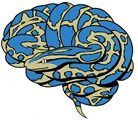
\includegraphics[width=3em]{nipylogo}} % No eye catcher for this poster. (eyecatcher=no above). If an eye catcher is present, the title is centered between eye-catcher and logo.
 % Title
  {\sf %Sans Serif
  %\bf% Serif
  Nipype: Opensource platform for unified and replicable\\ interaction
  with existing neuroimaging tools\vspace{0.15em}}
 {\centering\sf %Sans Serif
  % Serif
    SS Ghosh$^1$, C Burns$^2$, D Clark$^2$, K Gorgolewski$^3$, YO
    Halchenko$^4$, C Madison$^2$, R Tungaraza$^5$, KJ
    Millman$^2$\\
    \small\sf$^1$MIT, Cambridge, MA, USA $^2$U. California, Berkeley, CA, USA $^3$U. Edinburgh, UK
    $^4$Dartmouth College, Hanover, NH, USA $^5$U. Washington, Seattle, WA, USA\vspace{-0.4em}}

  % University logo
  % {% The makebox allows the title to flow into the logo, this is a hack because of the L shaped logo.
  %   \makebox[3em][r]{%
  %     \begin{minipage}{3em}
  %       \hfill
  %       %\includegraphics[height=2em]{msrlogo}
  %       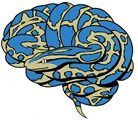
\includegraphics[height=3em]{nipylogo}
  %     \end{minipage}
  %   }
  % }

  \tikzstyle{light shaded}=[top color=baposterBGtwo!30!white,bottom color=baposterBGone!30!white,shading=axis,shading angle=30]

  % Width of left inset image
     \setlength{\leftimgwidth}{0.78em+8.0em}

%%%%%%%%%%%%%%%%%%%%%%%%%%%%%%%%%%%%%%%%%%%%%%%%%%%%%%%%%%%%%%%%%%%%%%%%%%%%%%
%%% Now define the boxes that make up the poster
%%%---------------------------------------------------------------------------
%%% Each box has a name and can be placed absolutely or relatively.
%%% The only inconvenience is that you can only specify a relative position 
%%% towards an already declared box. So if you have a box attached to the 
%%% bottom, one to the top and a third one which should be in between, you 
%%% have to specify the top and bottom boxes before you specify the middle 
%%% box.
%%%%%%%%%%%%%%%%%%%%%%%%%%%%%%%%%%%%%%%%%%%%%%%%%%%%%%%%%%%%%%%%%%%%%%%%%%%%%%
    %
    % A coloured circle useful as a bullet with an adjustably strong filling
    \newcommand{\colouredcircle}[1]{%
      \tikz{\useasboundingbox (-0.2em,-0.32em) rectangle(0.2em,0.32em); \draw[draw=black,fill=headerFontColor!80!black!#1!white,line width=0.03em] (0,0) circle(0.18em);}}
   \renewcommand{\labelitemi}{\colouredcircle{100}}
   \renewcommand{\labelitemii}{\colouredcircle{50}}

%%%%%%%%%%%%%%%%%%%%%%%%%%%%%%%%%%%%%%%%%%%%%%%%%%%%%%%%%%%%%%%%%%%%%%%%%%%%%%
  \headerbox{Introduction}{name=introduction,column=0,row=0}{
%%%%%%%%%%%%%%%%%%%%%%%%%%%%%%%%%%%%%%%%%%%%%%%%%%%%%%%%%%%%%%%%%%%%%%%%%%%%%%
    Current neuroimaging software offer users an incredible opportunity
    to analyze their data in different ways, with different underlying
    assumptions. However, this has resulted in a heterogeneous
    collection of specialized applications without transparent
    interoperability or a uniform operating interface. Nipype solves
    these issues by providing a uniform interface to existing
    neuroimaging software and by facilitating interaction between these
    packages within a single workflow.
 }

%%%%%%%%%%%%%%%%%%%%%%%%%%%%%%%%%%%%%%%%%%%%%%%%%%%%%%%%%%%%%%%%%%%%%%%%%%%%%%
  \headerbox{Problems}{name=problems,column=0,below=introduction}{
%%%%%%%%%%%%%%%%%%%%%%%%%%%%%%%%%%%%%%%%%%%%%%%%%%%%%%%%%%%%%%%%%%%%%%%%%%%%%%
    \begin{list}{\labelitemi}{\leftmargin=1em}
      \compresslist
      \item \textbf{Optimal workflows.} Integrating different packages is tedious. 
      \item \textbf{Developers nightmare.} No standard framework for
        disseminating tools across packages.
      \item \textbf{Knowledge distribution.} Training new personnel
        takes time.
      \item \textbf{Leveraging technology.} Many packages do not address
        computational efficiency.
      \item \textbf{Replicating research.} Method sections are often
        inadequate for replication.  
    \end{list}
}

%%%%%%%%%%%%%%%%%%%%%%%%%%%%%%%%%%%%%%%%%%%%%%%%%%%%%%%%%%%%%%%%%%%%%%%%%%%%%%
  \headerbox{Features}{name=features,column=0,below=problems}{
%%%%%%%%%%%%%%%%%%%%%%%%%%%%%%%%%%%%%%%%%%%%%%%%%%%%%%%%%%%%%%%%%%%%%%%%%%%%%%
    \begin{list}{\labelitemi}{\leftmargin=1em}
      \compresslist
    \item \textbf{Multi-package support.} Uniform cross-package
      interface (supports SPM, FSL, FreeSurfer components).
    \item \textbf{Minimal programming knowledge.} A high level scripting
      interface to design workflows intended for non-programmers.
    \item \textbf{Parallel execution.} No additional coding necessary
      for parallel execution of processing stages.
    \item \textbf{Pedagogical.} Can be used as a teaching tool and
      facilitates user training.
    \item \textbf{Well documented.} Code documentation becomes user
      documentation.
    \item \textbf{Shared workflows.} Workflows separate execution stages
      from data and can be shared within and across labs.  
    \end{list}
}

%%%%%%%%%%%%%%%%%%%%%%%%%%%%%%%%%%%%%%%%%%%%%%%%%%%%%%%%%%%%%%%%%%%%%%%%%%%%%%
  \headerbox{Component Architecture Diagram}{name=cad,column=1,span=2}{
%%%%%%%%%%%%%%%%%%%%%%%%%%%%%%%%%%%%%%%%%%%%%%%%%%%%%%%%%%%%%%%%%%%%%%%%%%%%%%
  \begin{tikzpicture}[x=\linewidth,y=\linewidth]
    %\path [use as bounding box] (-0.5,-0.5) rectangle(2.5,1.7);
    \node{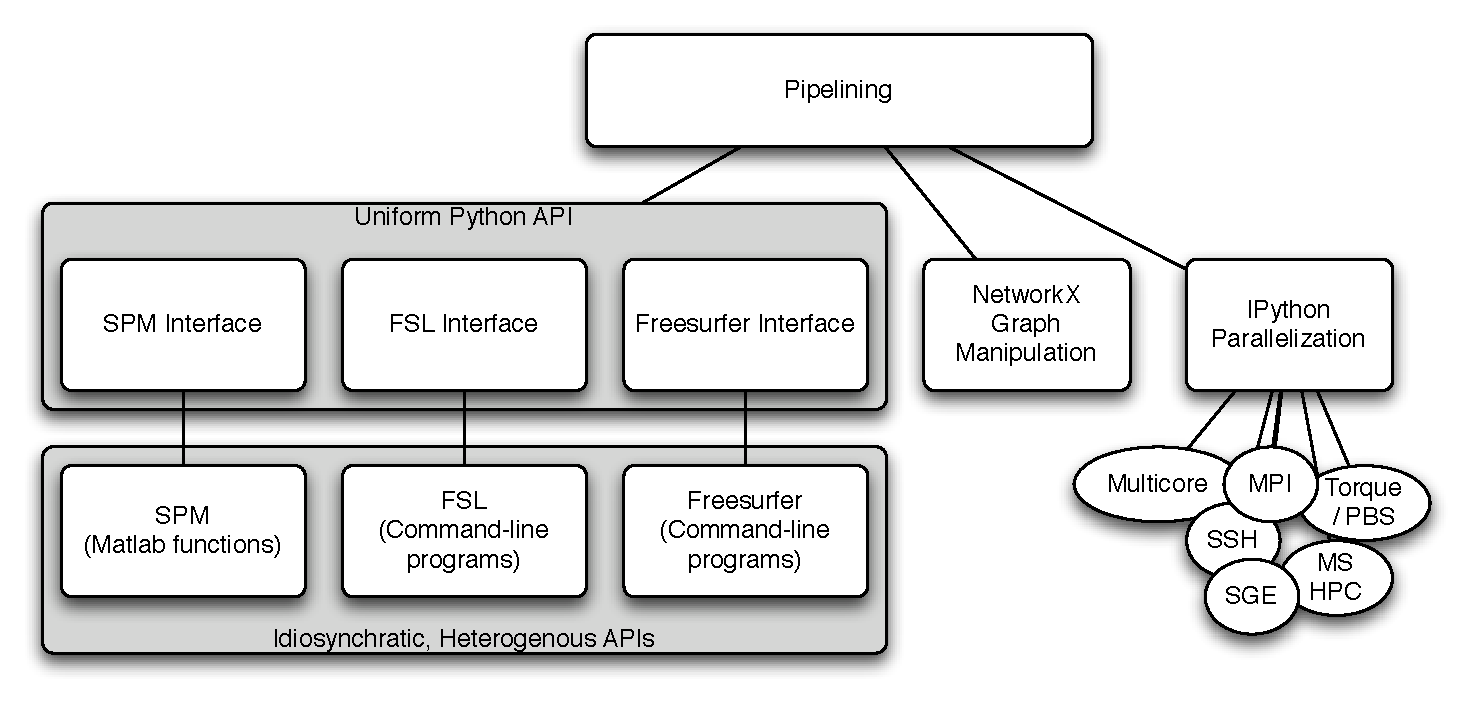
\includegraphics[width=\linewidth]{nipype_architecture}};
 \end{tikzpicture}
 }

\begin{SaveVerbatim}{InterfaceVerb}
In [5]: from nipype.interfaces.fsl import BET
In [6]: BET.help()

Inputs
------
Mandatory:
 in_file: input file to skull strip

Optional:
 args: Additional parameters to the command
 environ: Environment variables (default={})
 frac: fractional intensity threshold
 functional: apply to 4D fMRI data
  mutually exclusive: functional, reduce_bias
 mask: create binary mask image
...

Outputs
-------
out_file: path/name of skullstripped file
...

In [7]: bet = BET()
In [8]: res = bet.run(in_file='struct.nii', mask=True)
\end{SaveVerbatim}

%%%%%%%%%%%%%%%%%%%%%%%%%%%%%%%%%%%%%%%%%%%%%%%%%%%%%%%%%%%%%%%%%%%%%%%%%%%%%%
  \headerbox{Uniform package interface}{name=interface,column=1,below=cad}{
%%%%%%%%%%%%%%%%%%%%%%%%%%%%%%%%%%%%%%%%%%%%%%%%%%%%%%%%%%%%%%%%%%%%%%%%%%%%%%
    \UseVerbatim[fontsize=\relsize{-2.5}]{InterfaceVerb}
}

\begin{SaveVerbatim}{WorkflowVerbImport}
from nipype.pipeline.engine import (Workflow,
                                    Node, Mapnode)
from nipype.interfaces.spm import Realign
from nipype.interfaces.fsl import Smooth
\end{SaveVerbatim}

\begin{SaveVerbatim}{WorkflowVerbDefine}
realign = Node(interface=Realign(), name='realign')
smooth = MapNode(interface=Smooth(fwhm=6),
                 iterfield=['in_file'], name='smooth')
\end{SaveVerbatim}

\begin{SaveVerbatim}{WorkflowVerbConnect}
preproc = Workflow()
preproc.connect(realign, 'realigned_files',
                smooth, 'in_file')
\end{SaveVerbatim}

\begin{SaveVerbatim}{WorkflowVerbExecute}
preproc.inputs.realign.in_files = ['run1.nii', 'run2.nii']
preproc.base_dir = './workdir'
preproc.run()
\end{SaveVerbatim}

%%%%%%%%%%%%%%%%%%%%%%%%%%%%%%%%%%%%%%%%%%%%%%%%%%%%%%%%%%%%%%%%%%%%%%%%%%%%%%
  \headerbox{Simple workflow construction}{name=workflow,column=2,below=cad}{
%%%%%%%%%%%%%%%%%%%%%%%%%%%%%%%%%%%%%%%%%%%%%%%%%%%%%%%%%%%%%%%%%%%%%%%%%%%%%%
    \textbf{Import components}
    \vspace{-0.3em}
    \UseVerbatim[fontsize=\relsize{-2.5}]{WorkflowVerbImport}
    \vspace{-0.3em}
    \textbf{Define processes}
    \vspace{-0.3em}
    \UseVerbatim[fontsize=\relsize{-2.5}]{WorkflowVerbDefine}
    \vspace{-0.3em}
    \textbf{Construct workflow}
    \vspace{-0.3em}
    \UseVerbatim[fontsize=\relsize{-2.5}]{WorkflowVerbConnect}
    \vspace{-0.3em}
    \textbf{Execute workflow}
    \vspace{-0.3em}
    \UseVerbatim[fontsize=\relsize{-2.5}]{WorkflowVerbExecute}
}

%%%%%%%%%%%%%%%%%%%%%%%%%%%%%%%%%%%%%%%%%%%%%%%%%%%%%%%%%%%%%%%%%%%%%%%%%%%%%%
  \headerbox{Funding}{name=funding,column=1,above=bottom}{
%%%%%%%%%%%%%%%%%%%%%%%%%%%%%%%%%%%%%%%%%%%%%%%%%%%%%%%%%%%%%%%%%%%%%%%%%%%%%%
    \smaller This project was supported by NIH grants NIBIB R03 EB008673
    (PI: Ghosh, Whitfield-Gabrieli), NIMH R01 MH081909 (PI: D'Esposito).
  }

%%%%%%%%%%%%%%%%%%%%%%%%%%%%%%%%%%%%%%%%%%%%%%%%%%%%%%%%%%%%%%%%%%%%%%%%%%%%%%
  \headerbox{Hierarchical workflow visualization}{name=hierarchy,column=1,span=2,below=interface}{
%%%%%%%%%%%%%%%%%%%%%%%%%%%%%%%%%%%%%%%%%%%%%%%%%%%%%%%%%%%%%%%%%%%%%%%%%%%%%%
  \begin{tikzpicture}[x=\linewidth,y=\linewidth]
    %\draw[help lines] (0,0) grid (0.5,0.5);
    \node at (-0.2,0) {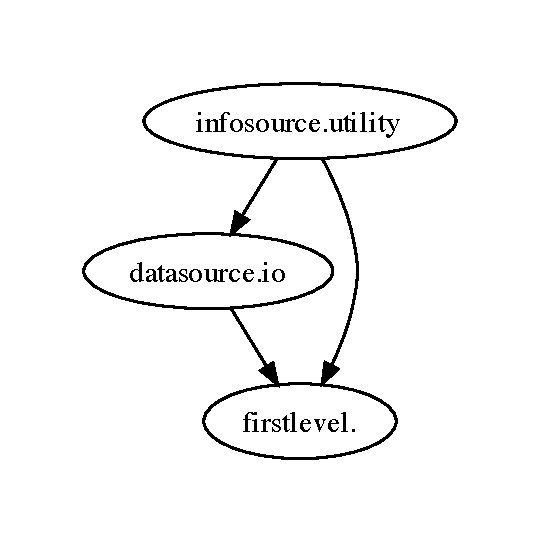
\includegraphics[width=0.2\linewidth]{level1}};
    \node at (0,0) {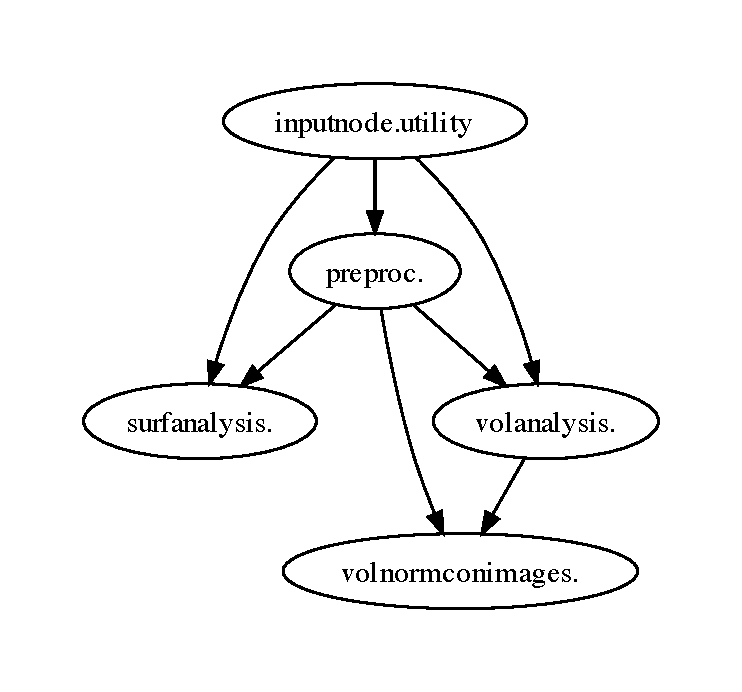
\includegraphics[width=0.3\linewidth]{firstlevel}};
    \node at (0.42,-0.01) {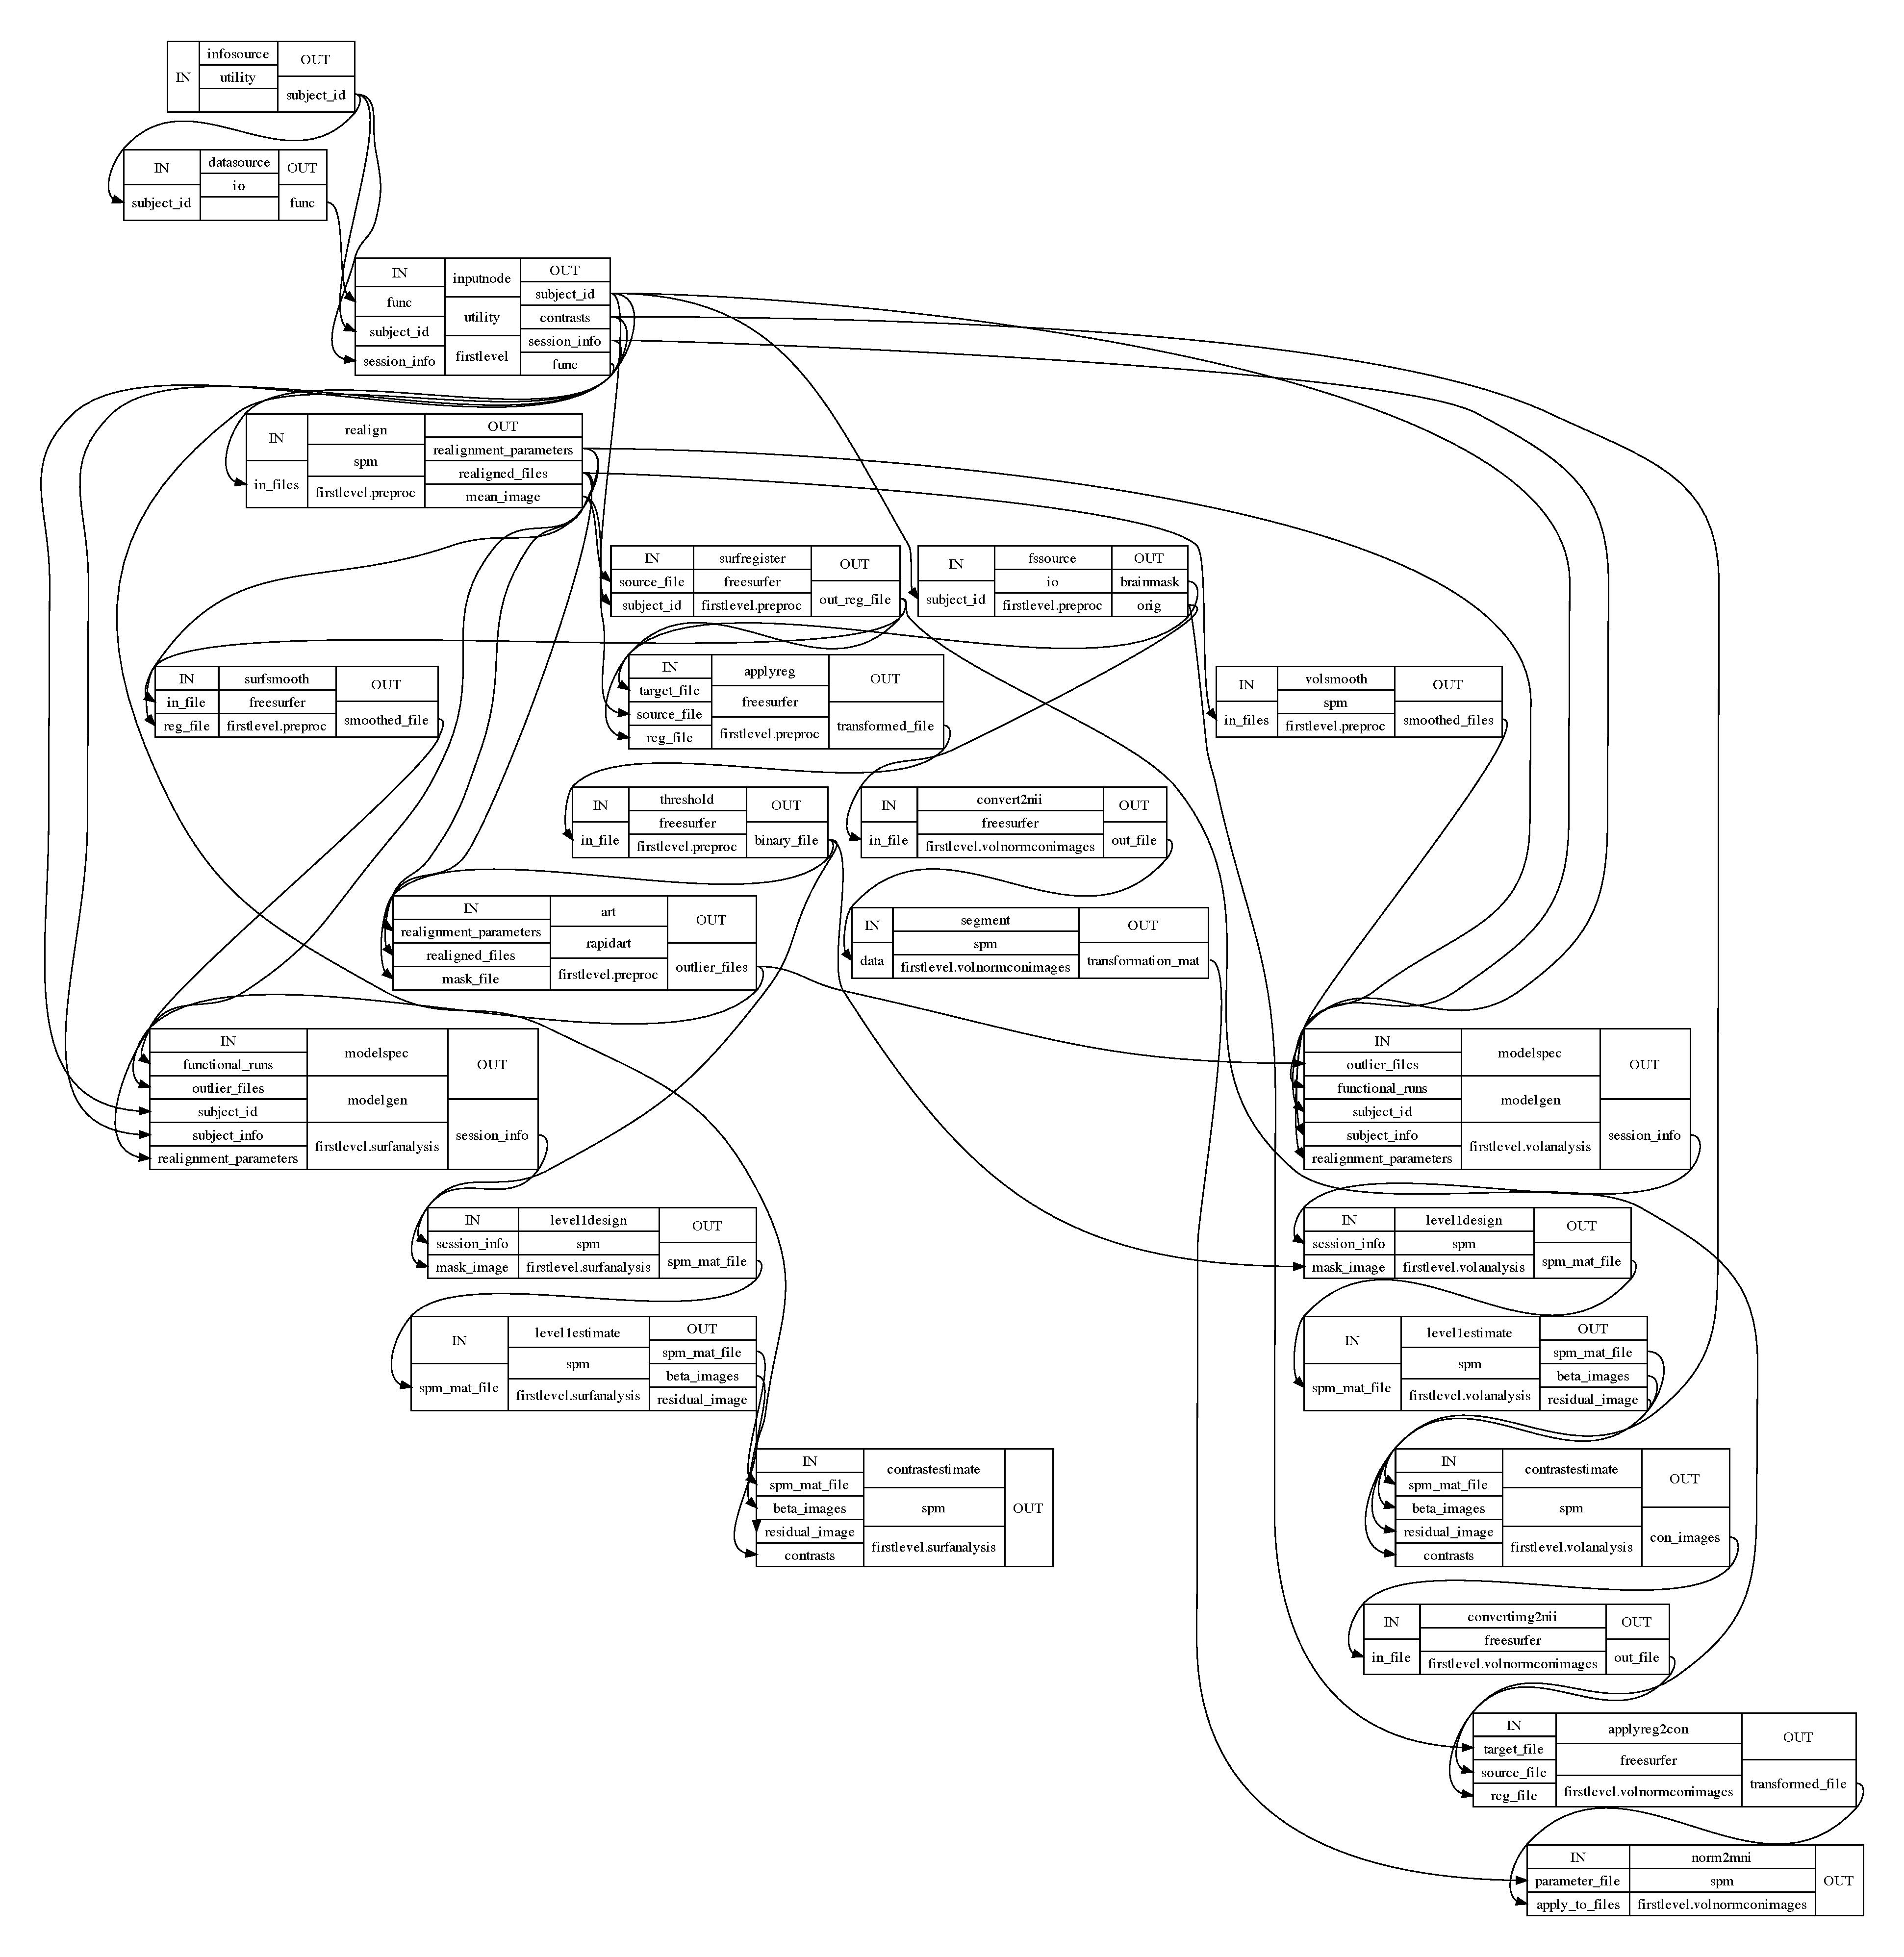
\includegraphics[width=0.6\linewidth]{detailed_graph}};
    \draw (0.13,-0.2) rectangle(0.71,0.2);
    \draw (0.18, 0.185) node(preproc) {preproc};
    \draw (-0.125,-0.2) rectangle(0.125,0.2);
    \draw (-0.075, 0.185) node(firstlevel) {firstlevel};
    \vspace{-2em}
 \end{tikzpicture}
}

%%%%%%%%%%%%%%%%%%%%%%%%%%%%%%%%%%%%%%%%%%%%%%%%%%%%%%%%%%%%%%%%%%%%%%%%%%%%%%
  \headerbox{Parallel execution}{name=parallel,column=1,below=hierarchy}{
%%%%%%%%%%%%%%%%%%%%%%%%%%%%%%%%%%%%%%%%%%%%%%%%%%%%%%%%%%%%%%%%%%%%%%%%%%%%%%
    \begin{list}{\labelitemi}{\leftmargin=1em}
      \compresslist
      \item Leverages IPython for distributed computation. 
      \item Non-dependent processes can be executed in parallel.
      \item No additional coding necessary.
      \item Example: SPM fMRI workflow on 69 subjects 
        \begin{list}{\labelitemi}{\leftmargin=2em}
          \compresslist
          \item Typical runtime: 3 days.
          \item Nipype runtime: 1 h 40 min on 40 cores.  
        \end{list}
    \end{list}
}

%%%%%%%%%%%%%%%%%%%%%%%%%%%%%%%%%%%%%%%%%%%%%%%%%%%%%%%%%%%%%%%%%%%%%%%%%%%%%%
  \headerbox{Future plans}{name=future,column=2,below=hierarchy}{
%%%%%%%%%%%%%%%%%%%%%%%%%%%%%%%%%%%%%%%%%%%%%%%%%%%%%%%%%%%%%%%%%%%%%%%%%%%%%% 
    \begin{list}{\labelitemi}{\leftmargin=1em}
      \compresslist
    \item \textbf{More interfaces.} 
      \begin{list}{\labelitemi}{\leftmargin=2em}
        \compresslist
        \item Complete coverage of existing packages.
        \item Newer registration algorithms (e.g., ANTS - U. Penn, CVS - MGH)
        \item Integration with tools in Nipy, Dipy and Nitime.
        \item Integrate with Slicer
      \end{list}
    \item \textbf{Web interface.} A graphical interface to define workflows.
    \item \textbf{Workflow repository.} Create a centralized location
      for version controlled workflows.
    \item \textbf{Additional modalities.}  Extend to PET, EEG/MEG,
      fNIRS.
    \end{list}

}

%%%%%%%%%%%%%%%%%%%%%%%%%%%%%%%%%%%%%%%%%%%%%%%%%%%%%%%%%%%%%%%%%%%%%%%%%%%%%%
  \headerbox{Sotware dependencies}{name=software,column=0,above=bottom}{
%%%%%%%%%%%%%%%%%%%%%%%%%%%%%%%%%%%%%%%%%%%%%%%%%%%%%%%%%%%%%%%%%%%%%%%%%%%%%%
    \smaller
   \begin{tabular}{rl}
     Nipy & \url{nipy.sourceforge.net}\\
     Ipython & \url{ipython.scipy.org}\\
     Scipy,Numpy & \url{scipy.org}\\
     Networkx & \url{networkx.lanl.gov}\\
     NeuroDebian & \url{neuro.debian.net}\\
     Traits & \url{www.enthought.com}
   \end{tabular}

 }

%%%%%%%%%%%%%%%%%%%%%%%%%%%%%%%%%%%%%%%%%%%%%%%%%%%%%%%%%%%%%%%%%%%%%%%%%%%%%%
  \headerbox{Conclusion}{name=conclusion,column=0,span=1,below=features,above=software}{
%%%%%%%%%%%%%%%%%%%%%%%%%%%%%%%%%%%%%%%%%%%%%%%%%%%%%%%%%%%%%%%%%%%%%%%%%%%%%%
    \begin{list}{\labelitemi}{\leftmargin=1em}
      \compresslist
    \item Provides an environment for interactive manipulation of data
      through a Python interface as well as for performing reproducible,
      distributed analysis using a pipeline system.
    \item Encourages scientific exploration of different algorithms and
      associated parameters.
    \item Simplifies the development of workflows within and between
      packages.
    \item Reduces the learning curve associated with understanding the
      algorithms, APIs and user interfaces of disparate packages.
    \end{list}
   \begin{tabular}{rl}
     Engages the community & \textbf{C}ollaborative\\
      Available for all & \textbf{O}pensource\\
      Workflows are records & \textbf{R}eproducible\\
      Minimizes redundancy & \textbf{E}fficient
    \end{tabular}
}

\end{poster}%
\end{document}
